\chapter{Existujúce riešenia}\label{chap:riesenia}
Napriek vzrastajúcej popularite voxelovej grafiky neexistuje doposiaľ mnoho kvalitných nástrojov na ich editáciu. Preto sme vybrali niektoré z nich, ktoré nám svojim charakterom najviac vyhovujú. 
Celkovo môžme rozdeliť takéto programy do dvoch skupín. Jednou sú programy slúžiace na digitálne sochárstvo s voxelovým základom a druhou sú nástroje zámerne zobrazujúce každý voxel.

\section{Digitálne sochárstvo}
Digitálne sochárstvo je pomerne nová a zaujímavá metóda 3D modelovania. Umožňuje pridávanie najjemnejších detajlov a v prípade voxelových programov aj bez ohľadu na topológiu modelu. Vďaka tomu aj napriek pomerne krátkej existencii sa táto metóda stala veľmi populárnou medzi tvorcami detajlnej 3D grafiky. Voxelové sochárstvo sa prevažne využíva na tvorbu modelov s fotorealistickým až hyperrealistickým vzhľadom, ktoré slúžia ako predlohy do filmov, hier, priemyselného dizajnu a taktiež ako realistické ilustrácie a podobne. Nechceme sa však zamerať na tento smer modelovania, keďže nevyužíva voxely ako základnú stavebnú jednotku, ale len ako nástroj k zlepšeniu detajlov modelov alebo ako nástroj umožňujúci slobodnejšiu tvorbu.

Zoznam zaujímavých voxel-based programov pre digitálne sochárstvo:
\begin{itemize}
	\item \textbf{3Dcoat} Program, ktorý zadefinoval pojem \textit{Voxel Sculpting}.
	\item \textbf{Acropora} Procedurálny voxelový modeler.
	\item \textbf{Crysis Terrain editor} Program na tvorbu členitých terénov do počítačovej hry \textit{Crysis}.
\end{itemize}

\section{Editory voxelovej grafiky}
V tejto časti sa zameriavame na programy, ktoré na rozdiel od nástrojov na digitálne sochárstvo nevyužívajú voxely len ako pomôcku k dosiahnutiu detajlného výsledku s pomerne vysokým levelom slobody tvorby, ale ako primárnu stavebnú jednotku 3D objektov. Takéto nástroje neumožňujú veľké rozlíšenia voxelových priestorov a teda nie sú ani zamerané na detajl modelov. Toto spôsobuje, že užívateľ má pod kontrolou každý voxel scény, ale aj to, že sú viditeľné rôzne artefakty, obzvlášť zubatý okraj objektov. Takýto stav nemožno nazvať nevýhodou, keďže mnoho fanúšikov voxelov ostré hrany obľubuje, pretože práve viditeľné kocky dodávajú voxelovej grafike to správne čaro.

Nasledujúci prehľad obsahuje vzorku voxelových editorov, ktoré sa nám podarilo nainštalovať a korektne spustiť. Taktiež obsahuje ich stručný opis s výhodami a nevýhodami, ktoré sme zaznamenali pri krátkom testovaní.
\subsection{Paint3D}
Daný program predstavuje jednoduchú 3D alternatívu pre program MS Paint \cite{paint3d}. Interface aplikácie je zobrazený na obrázku \ref{obr:paint3D}.
\subsubsection{Výhody:}
\begin{itemize}
	\item \textbf{Jednoduchosť}. Na webovej stránke tohoto programu tvorcovia proklamujú, že je nástroj jednoduchý na používanie. Do istej miery je to aj pravda, avšak pri testovaní sme museli využiť niektoré internetové zdroje, aby sme pochopili, ako program funguje. 
	\item \textbf{Nástroje}. V ponuke sú rôzne užitočné nástroje a je ich taktiež primerané množstvo.
	\item \textbf{Priehladnosť}. Program podporuje, ako jediný z testovaných, alfa transparenciu voxelov.
	\item \textbf{Spolupráca sa 2D grafickými programami}. Tento nástroj umožňuje funkcie copy/paste z iných 2D grafických programov, ako je napríklad MS Paint od spoločnosti \textit{Microsoft}.
	\item \textbf{Kresliace módy}. Program ponúka viaceré módy kreslenia voxelov. Či už po rezoch v rôznych osiach alebo priestorovým kreslením štetcom s nastaviteľnou hrúbkou.
	\item \textbf{Export/Import}. Program podporuje široké množstvo voxelových formátov.
	\item \textbf{Skriptovanie}. Asi najväčšou výhodou tohto nástroja je skriptovanie, ktoré sa dá v grafike a vo voxelovej obzvlášť dobre využiť pri tvorbe inak pracne vytvorených modelov.  
\end{itemize}

\subsubsection{Nevýhody:}
\begin{itemize}
	\item \textbf{Zahlcovanie procesora}. Program už pri spustení a počas celého behu vyťaží procesor na takmer 100\%. Toto by nemal robiť žiaden rozumný program pri pokojovom stave.
	\item \textbf{Plná verzia je platená}. Ak by ste chceli využívať všetky možnosti programu, musíte si priplatiť 20\$. Našťastie je trial verzia voľne stiahnuteľná a to, čo ponúka je dostačujúce na prácu.
	\item \textbf{Jeden objekt v scéne.} Možnosť pridávania viacerých objektov do scény neumožňuje väčšina programov.
\end{itemize}
\begin{figure}[ht!]
	\centering
	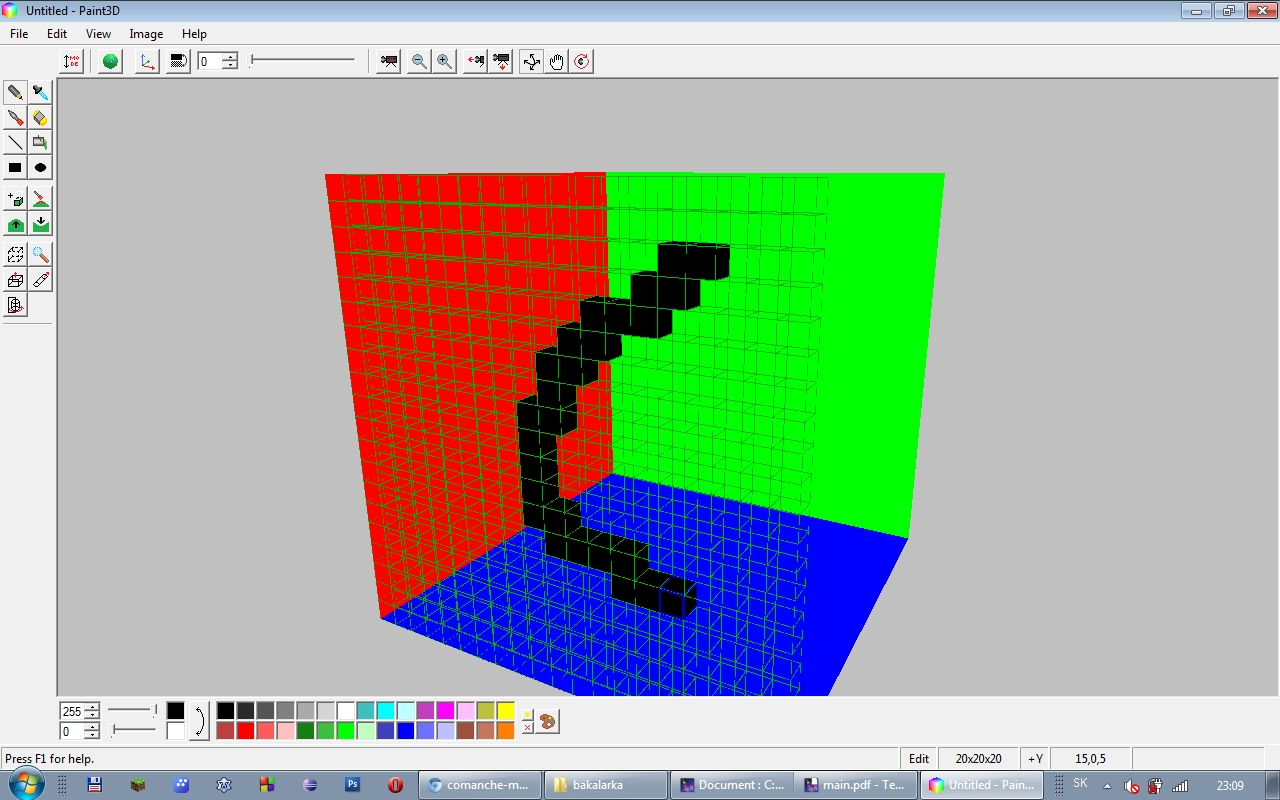
\includegraphics[width=0.8\textwidth]{paint3D.jpg}
	\caption[Paint3D]{Screenshot z programu Paint3D}
	\label{obr:paint3D}
\end{figure}


\subsection{Voxel3D}
Jedná sa o program od spoločnosti \textit{Everygraph} \cite{voxel3d}. Interface aplikácie je zobrazený na obrázku \ref{obr:voxel3D}.
\subsubsection{Výhody:}
\begin{itemize}
	\item \textbf{Voxelizácia}. Ako jediný z testovaných ponúka možnosť voxelizície 3D meshu. Taktiež umožňuje počas tvorby zobraziť tento mesh spolu s voxelizovaným objektom a podľa ľubovôle ho umiestňovať. 
	\item \textbf{Jednoduchý interface}. V programe sa dá ľahko zorientovať, a preto je vhodný aj pre neskúsených užívateľov.
	\item \textbf{4 rôzne náhľady}. Táto funkcionalita je bežná v 3D modelovacích nástrojoch, avšak toto je jediný z testovaných voxelových editorov, ktorý ju obsahuje.
	\item \textbf{Import/Export}. Výhodou programu je, že má vlastný binárny a aj ASCII formát na ukladanie dát. Taktiež program ponúka aj export do .obj formátu. Nevýhodou však je, že program nepodporuje žiadne iné bežne používané voxelové formáty.
\end{itemize}
\subsubsection{Nevýhody:}
\begin{itemize}
	\item  \textbf{Rýchlosť}. Tento parameter dosahuje nedostatočné hodnoty najmä pri vytváraní prázdneho objektu. Už pri pomerne malých rozmeroch vytvorenie objektu trvá iritujúco dlho. Pri testovaní sme vytvárali objekt s počtom voxelov \begin{math}32^3\end{math} a ďalší objekt mal počet voxelov \begin{math}64^3\end{math}. Vytvorenie prvého objektu trvalo približne 6 sekúnd, zatiaľ čo vytvorenie druhého trvalo približne 48 sekúnd.
	\item \textbf{Neošetrené vstupy}. Napriek tomu, že je program pomalý aj pri malých rozmeroch, jeho interface umožňuje vytvoriť objekt s počtom voxelov \begin{math}(2^{32})^3\end{math}.
	\item \textbf{Zdĺhavé modelovanie}. Očakávame, že tvorba voxelových objektov nebude najrýchlejšia, avšak kreslenie voxelov v tomto programe je o to zdĺhavejšie, že umožňuje kresliť iba po rezoch objektom.
	\item \textbf{Jeden objekt v scéne.} Možnosť pridávania viacerých objektov do scény neumožňuje väčšina programov.
\end{itemize}

\begin{figure}[ht!]
	\centering
	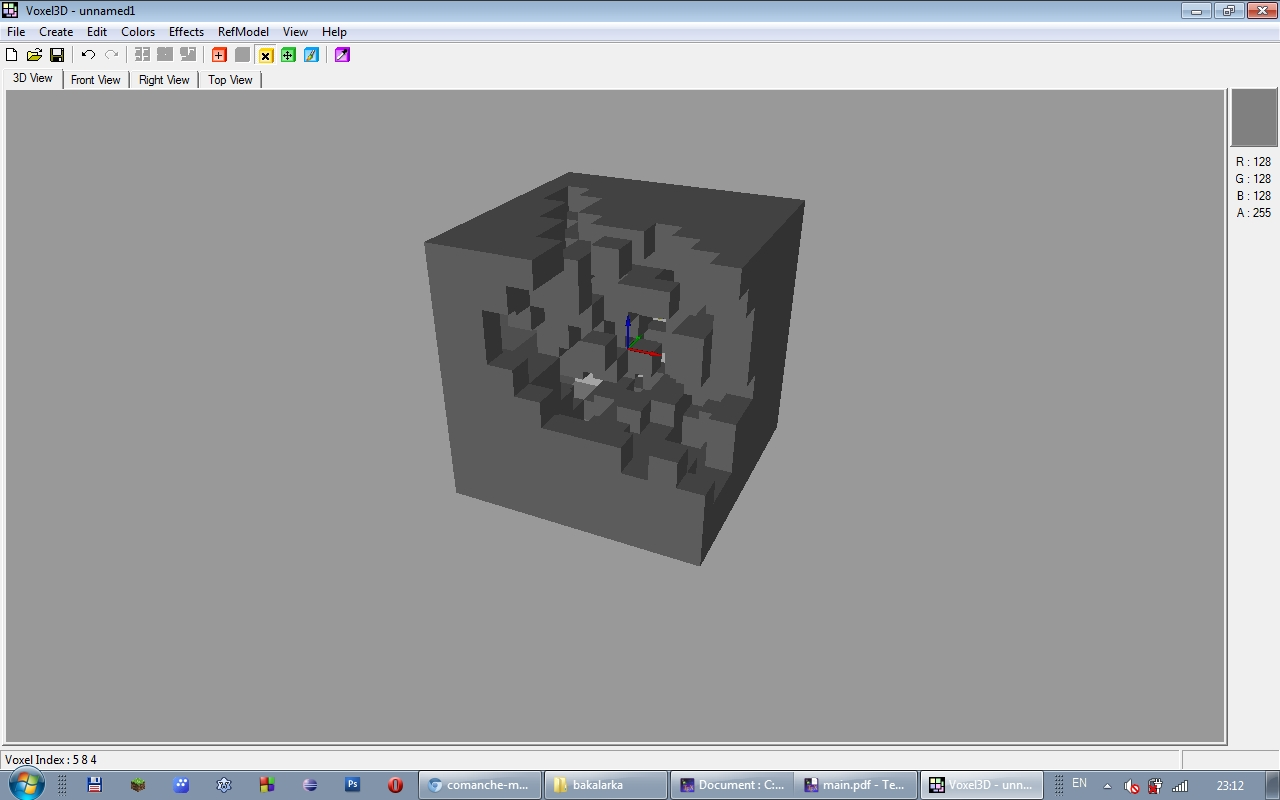
\includegraphics[width=0.8\textwidth]{Voxel3D.jpg}
	\caption[Voxel3D]{Screenshot z programu Voxel3D}
	\label{obr:voxel3D}
\end{figure}

\subsection{3D Dot Game Hero Editor}
Táto aplikácia je skôr online editor, pre tvorbu voxelových hrdinov do hry 3D Dot Game \cite{dotGame}. Interface aplikácie je zobrazený na obrázku \ref{obr:hero}.
\subsubsection{Výhody:}
\begin{itemize}
	\item \textbf{Dostupnosť cez prehliadač}. Tento fakt je aj výhodou, ale aj nevýhodou daného programu, pretože je dostupný výlučne cez prehliadač a neexistuje desktopová verzia.
	\item \textbf{Jednoduchosť použitia}. Táto vlastnosť je zaručená najmä vďaka malému množstvu nástrojov a možností softvéru.
	\item \textbf{Render a animácia}. Ak v programe zvolíme možnosť \textit{save}, automaticky sa vyrenderuje balík výstupných súborov, ktoré sa nám ponúknu na stiahnutie. Tento balík obsahuje 2 rendery s pozadím a bez pozadia, jednu animáciu objektu (ide iba o rotáciu okolo vlastnej osi) a jeden wallpaper. 
\end{itemize}

\subsubsection{Nevýhody:}
\begin{itemize}
	\item \textbf{Ponuka nástrojov}. Ako bolo spomenuté, program ponúka iba chudobné množstvo editovacích nástrojov v počte 3.
	\item \textbf{Obmedzenie farieb}. Taktiež aj farebná paleta je obmedzená na niečo viac ako tucet farebných odtieňov.
	\item \textbf{Obmedzené rozmery}. Tvorený objekt je ohraničený bounding boxom, ktorý nemožno nijak prekročiť, ani zmeniť jeho rozmery.
	\item \textbf{Export/Import}. V ponuke aplikácie nie je žiaden import a exportovať je možné iba render, ako bolo spomenuté vyššie.
	\item \textbf{Jeden objekt v scéne.} Možnosť pridávania viacerých objektov do scény neumožňuje väčšina programov.
\end{itemize}

\begin{figure}[ht!]
	\centering
	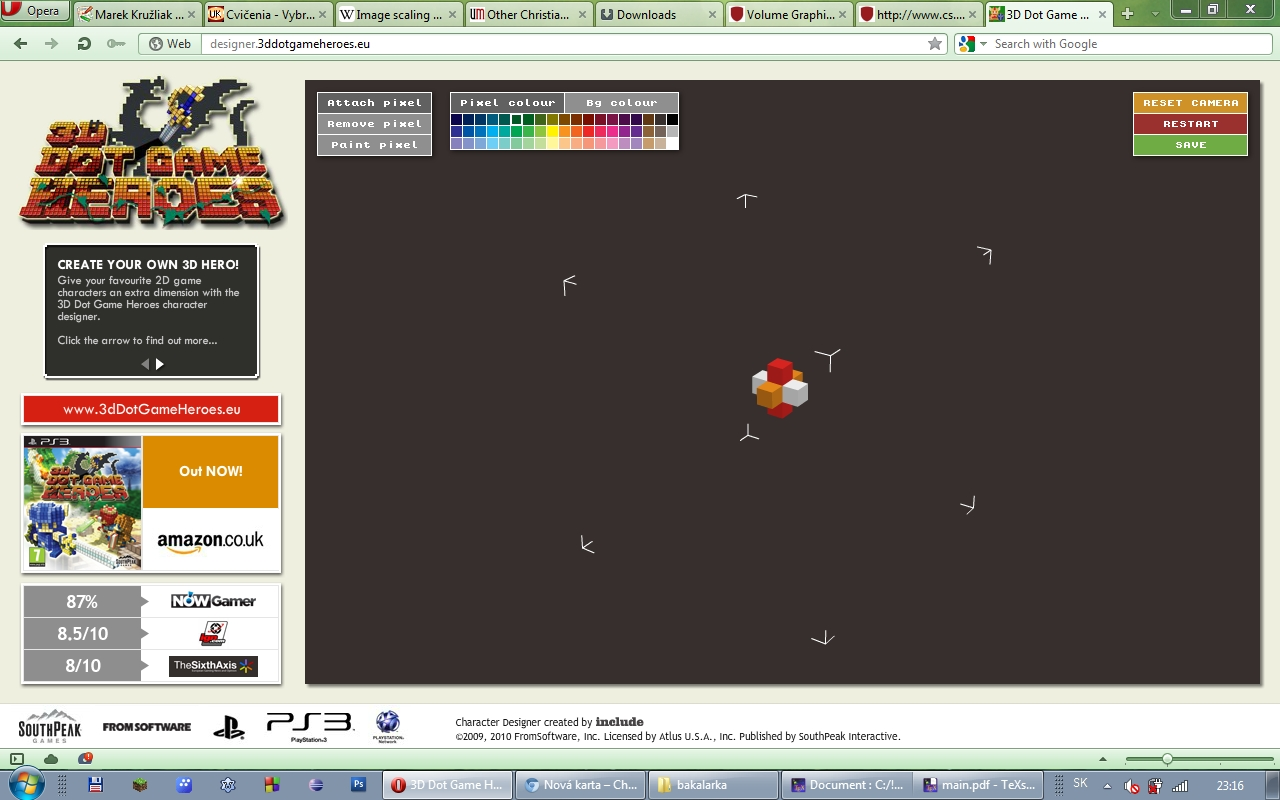
\includegraphics[width=0.8\textwidth]{3Dhero.jpg}
	\caption[3D Dot Game Hero Editor]{Screenshot z programu 3D Dot Game Hero Editor}
	\label{obr:hero}
\end{figure}


\subsection{Zoxel}
Zoxel je kvalitný výtvor od jediného človeka menom Graham King \cite{zoxel}. Interface aplikácie je zobrazený na obrázku \ref{obr:zoxel}.
\subsubsection{Výhody:}
\begin{itemize}
	\item \textbf{Lepší shading}. Väčšina programov používa pre tieňovanie jednoduchý flat-shading zatiaľ, čo Zoxel má implementovaný istý druh smooth-shadingu, resp. využíva základný z možností OpenGL knižnice.
	\item \textbf{Jednoduchý interface}. Interface je jednoduchý a intuitívny s možnosťou ľubovolného premiestňovania niektorých komponentov, ako napríklad paleta farieb alebo nástrojov.
	\item \textbf{Wireframe}. Program umožňuje zobraziť model ako wireframe.
	\item \textbf{Interaktívne rozširovanie voxelového priestoru}.
	\item \textbf{Import/Export}. Výhodou programu je, že má vlastný binárny formát na ukladanie dát. Taktiež program ponúka aj export do .obj formátu a ukladanie a náčítanie súboru z programu Sproxel spomenutého nižšie.
\end{itemize}
\subsubsection{Nevýhody:}
\begin{itemize}
	\item \textbf{Kamera}. Pri testovaní nám najväčšie problémy spôsobovala nemotorná kamera, ktorá občas prejavovala neočakávané správanie.
	\item \textbf{Kreslenie}. Kreslenie je vyriešené veľmi nešťastne, kedže sa dá pridať iba jeden voxel na klik. Teda nie je umožnené kreslenie na udalosť ťahania myši.
	\item \textbf{Chudobná ponuka nástrojov}.
	\item \textbf{Jeden objekt v scéne.} Možnosť pridávania viacerých objektov do scény neumožňuje väčšina programov.
\end{itemize}

\begin{figure}[ht!]
	\centering
	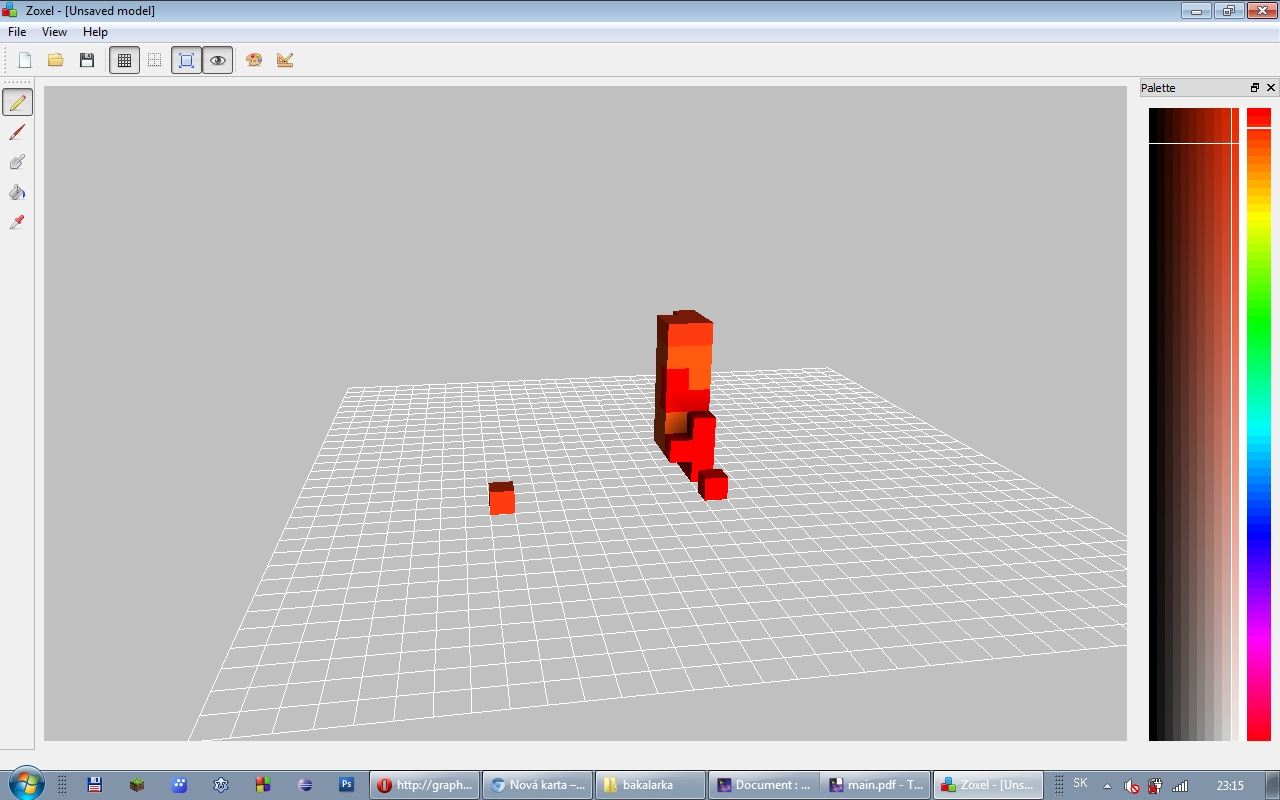
\includegraphics[width=0.8\textwidth]{zoxel.jpg}
	\caption[Zoxel]{Screenshot z programu Zoxel}
	\label{obr:zoxel}
\end{figure}

\subsection{Sproxel}
Horlivo vyvíjaný voxelový editor, tak by sa dal charakterizovať Sproxel \cite{sproxel}. Interface aplikácie je zobrazený na obrázku \ref{obr:sproxel}.
\subsubsection{Výhody:}
\begin{itemize}
	\item \textbf{Jednoduché ovládanie}. Program mal jedno z najlepších ovládaní a nebolo vôbec zložité sa ho naučiť.
	\item \textbf{Jednoduchý interface}. Interface je jednoduchý a intuitívny s možnosťou ľubovoľného premiestňovania niektorých komponentov, ako napríklad paleta farieb alebo nástrojov.
	\item \textbf{Ponuka nástrojov}. Ponuka nástrojov a rôznych úprav je dostačujúca a v porovnaní s niektorými programami až nadpriemerná.
	\item \textbf{Export/import}. Okrem vlastného binárneho súborového formátu na ukladanie a načítavanie objektov má aplikácia v ponuke aj rôzne druhy importu a exportu napríklad ako .obj alebo ako obrázok vo formáte .png a mnohé iné.
	\item \textbf{Medziplatformovosť}. 
	\item \textbf{Aktívny vývoj}. Aj v súčasnosti sa aktívne pracuje na vývoji tohto softvéru. Najnovšia verzia je Sproxel 0.6, takže nám vývojári pravdepodobne sľubujú ešte niekoľko ďalších verzií.
\end{itemize}
\subsubsection{Nevýhody:}
\begin{itemize}
	\item \textbf{Z-fighting}. Problém z-fightingu nie je riešený ani na miestach, kde by to bolo pomerne jednoduché. Jeho neriešenie spôsobuje nie len neestetickosť výsledku ale aj neprehľadnosť pri práci s voxelmi.
	\item \textbf{Voxel grid}. Čo by mohlo byť výhodou, je však nevýhodou, pretože zapnutie zobrazenia voxel gridu spôsobuje v podstate zaseknutie programu už pri počte voxelov \begin{math}32^3\end{math}.
	\item \textbf{Jeden objekt v scéne.} Možnosť pridávania viacerých objektov do scény neumožňuje väčšina programov.
\end{itemize}

\begin{figure}[ht!]
	\centering
	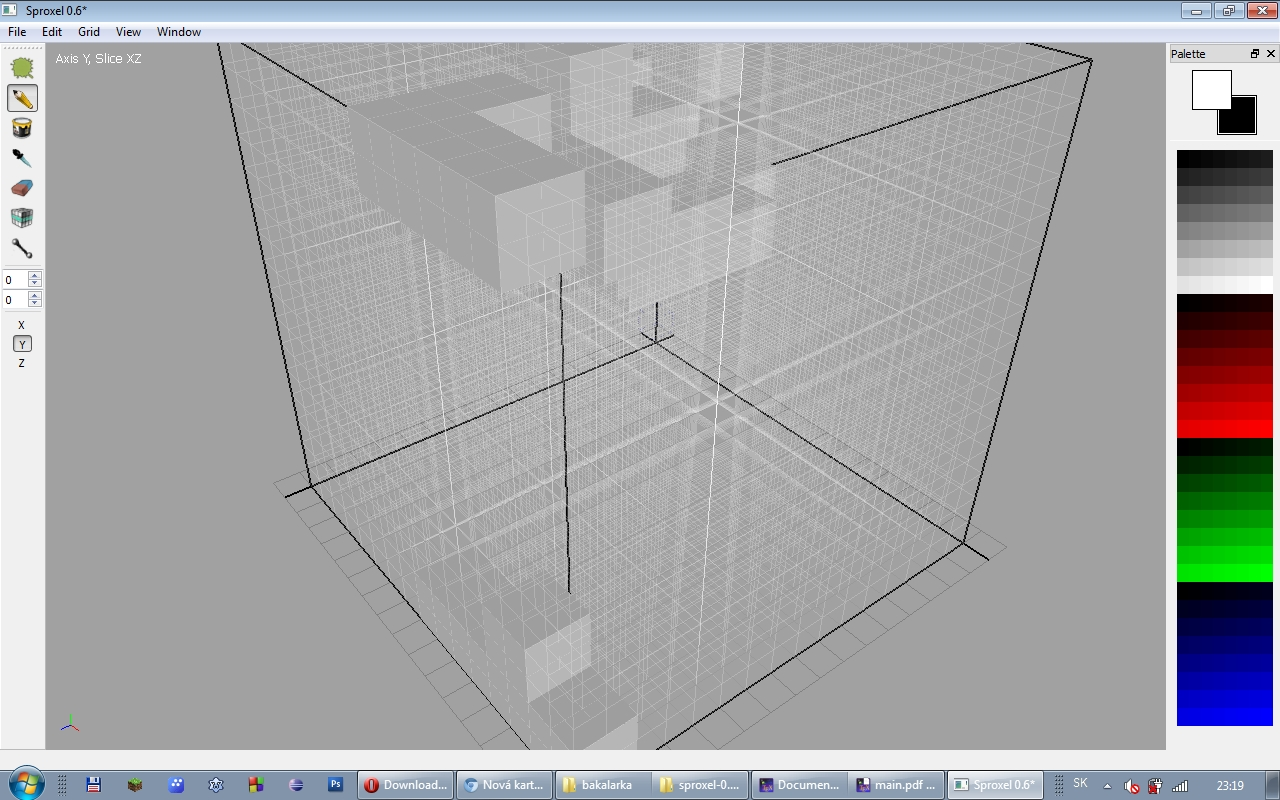
\includegraphics[width=0.8\textwidth]{sproxel.jpg}
	\caption[Sproxel]{Screenshot z programu Sproxel}
	\label{obr:sproxel}
\end{figure}

\eject

\subsection{Qubicle}
Qubicle je veľmi kvalitný softvér od spoločnosti minddesk \cite{qubicle}. Interface aplikácie je zobrazený na obrázku \ref{obr:qubicle}.
\subsubsection{Výhody:}
\begin{itemize}
	\item \textbf{Ponuka nástrojov a funkcií}. Aplikácia sama o sebe neponúka veľké množstvo nástrojov, avšak ich počet je dostačujúci a sú doplnené ohromným množstvom funkcií a nastavení na úpravu objektov a scén.
	\item \textbf{Interface.} Prostredie je pomerne jednoduché s obzvlášť peknou grafikou.
	\item \textbf{Viacej objektov v scéne}. Tento program ako jediný z testovaných ponúka možnosť vytvárania viacerých nezávislých objektov v scéne, čo umožňuje lepšiu variabilnosť pri tvorbe.
	\item \textbf{Defaultné tvary}. Okrem prázdneho objektu je možné pridať základné objemové útvary ako napríklad kváder, ihlan, elipsoid, valec a kužel. Taktiež je možné vygenerovať náhodný voxelový terén. Táto možnosť je však až v platenej verzii, preto sme ju nemohli otestovať.
	\item \textbf{Editačné módy}. Rozličné módy editovania nám umožňujú tvoriť na troch rozličných leveloch. Na úrovni scény, na úrovni objektu a na úrovni rezu. Vďaka tomu máme pomerne veľkú kontrolu nad tým, čo robíme. 
	\item \textbf{Import/Export}. Program má vlastný binárny formát na ukladanie a na načítavanie súborov. Taktiež je možný export do XML, .obj alebo do rôznych známych binárnych voxelových formátov.
	\item \textbf{Lokalizácia}. V nastaveniach programu je možné vybrať jeden zo štyroch svetových jazykov.
	\item \textbf{Rendering}. Ako jeden z mála programov, má \textit{Quibicle} zabudovaný jednoduchý rendering objektov s obrázkovým súborom ako výstupom.
\end{itemize}
\subsubsection{Nevýhody:}
\begin{itemize}
	\item \textbf{Licencia}. Voľne stiahnuteľná je iba \textit{Basic} verzia programu, ktorá sa dá použiť výlučne na nekomerčné účely. Táto verzia nezahŕňa širšiu funkcionalitu a export objektov. Vyššie verzie sú platené.
	\item \textbf{Komplikovanosť}. Veľké množstvo funkcií a nastavení vyžaduje viacej času naučiť sa dokonale ovládať tento nástroj. Avšak základy je veľmi ľahké pochytiť a sú dostačujúce na dosiahnutie pomerne dobrých výsledkov.
\end{itemize}

\begin{figure}[ht!]
	\centering
	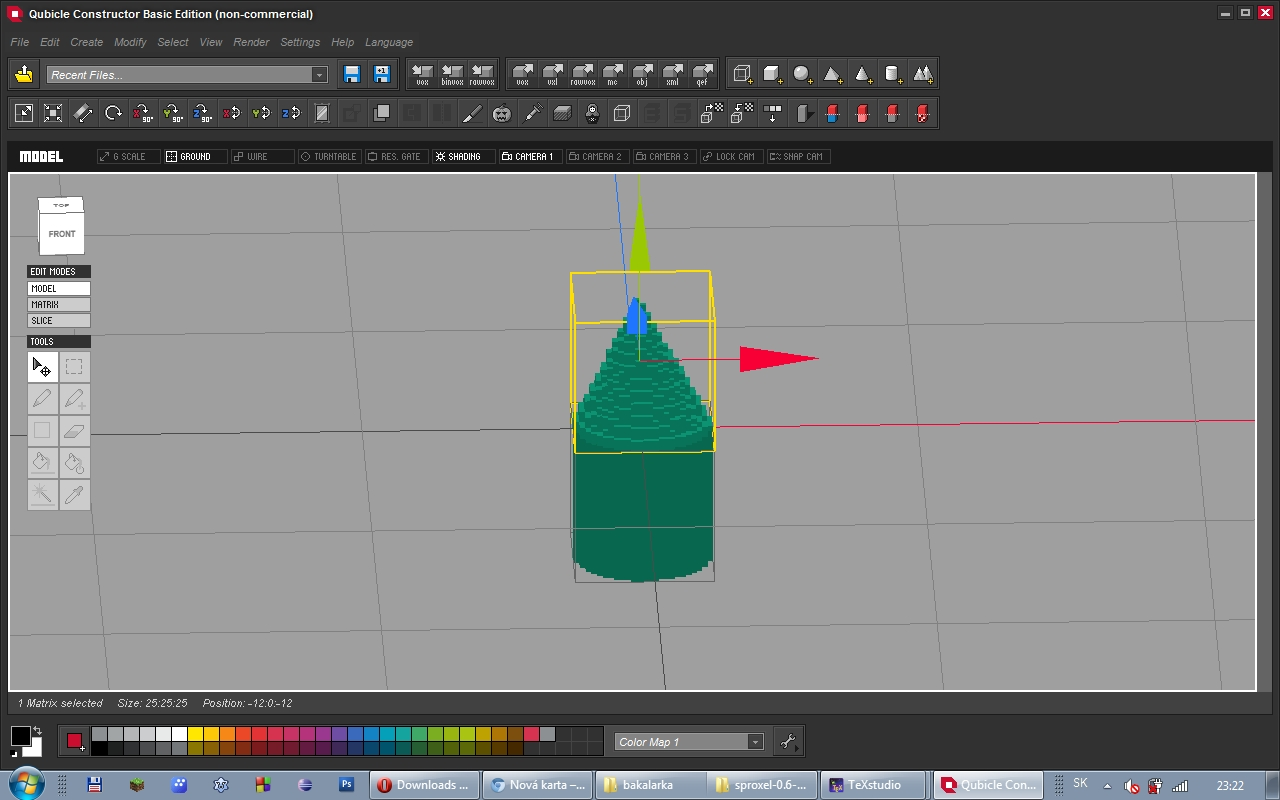
\includegraphics[width=0.8\textwidth]{qubicle2.jpg}
	\caption[Qubicle]{Screenshot z programu Qubicle}
	\label{obr:qubicle}
\end{figure}

\section{2D grafické editory}
Keďže si predstavujeme prácu s voxelmi ako kreslenie objektov v priestore, inšpiráciou nám pre našu prácu bolo mnoho 2D kresliacich programov akými sú napríklad \textit{Adobe Photoshop}, \textit{Gimp} alebo jednoduchší \textit{Microsoft Paint}. Tieto aplikácie poskytujú užívateľovi širokú sadu nástrojov, z ktorých sme sa rozhodli niektoré z nich použiť aj my. Taktiež sme sa snažili pri vytváraní GUI a nastavovaní spôsobu používania nástrojov vytvoriť podobný pocit, ako pri práci napríklad v programe MsPaint.

\section{Zhrnutie poznatkov z testovania}
Prieskum spomínaného softvéru nám umožnil vytvoriť si detajlnejší obraz o našich cieľoch a možnostiach pri implementácii práce. 
Najlepšie výsledky v testovaní dosiahol jednoznačne program Qubicle. Jeho filozofiou modelovania sme sa najväčšmi stotožnili, kedže ako jediný umožňoval vytvárať samostatné objekty, ktoré bolo následne možné ľubovoľne umiestniť v scéne. Taktiež obsahoval najväčšie množstvo funkcií a aj napriek tomu mal rýchlo pochopiteľný interface. Jeho najslabšou stránkou teda zostáva, že jeho plná verzia je platená.
Zvyšné programy nedosahovali podobné výsledky, avšak vytvorili spodnú hranicu kvality, ktorú by chcela dosiahnuť aj táto práca.


